\section{Einleitung}
Ein fundamentales Konzept in den Wirtschaftswissenschaften ist die von Frank H. Knight eingeführte Unterscheidung zwischen Risiko und 
Unsicherheit. Knight definierte Risiko als quantifizierbare Unsicherheit, also Situationen, in denen den möglichen Ergebnissen 
Wahrscheinlichkeiten zugeordnet werden können. Ein klassisches Beispiel hierfür sind Versicherungen oder Glücksspiele, bei denen 
aufgrund historischer Daten oder mathematischer Modelle die Wahrscheinlichkeiten der verschiedenen Ausgänge bekannt sind.

Unsicherheit hingegen, die Knight als "echte Unsicherheit" bezeichnet, bezieht sich auf Situationen, in denen diese Zuordnung nicht 
möglich ist. Dies tritt auf, wenn keine verlässlichen historischen Daten zur Verfügung stehen, um die Wahrscheinlichkeiten der 
verschiedenen Ergebnisse zu prognostizieren. Ein Beispiel hierfür wäre die Einführung eines innovativen Produkts auf den Markt, bei 
dem es keine vorherigen Daten gibt, die den Erfolg oder Misserfolg vorhersagen könnten. \cite{Knight1921}

Wenn man Unsicherheit aus der Perspektive der Datenvisualisierung betrachtet, stößt man auf viele ähnliche, jedoch auch zahlreiche 
unterschiedliche Definitionen. Haber und McNabb \cite{Haber1990} beschreiben einen generischen Prozess zur Visualisierung von Daten, 
der die verschiedenen Stufen von der Datenbeschaffung bis zur finalen Visualisierung abdeckt. Dieser Prozess, der auch von Pang et al. \cite{Pang1997} 
aufgegriffen wird, besteht aus mehreren Schritten, in denen Unsicherheit in unterschiedlichem Maße eingeführt und berücksichtigt
werden muss, und diese unterschiedlichen Definitionen verdeutlicht:

\begin{enumerate}
    \item \textbf{Datenbeschaffung}:
    In dieser Phase ist Unsicherheit inherent, sei es durch Messfehler/-ungenauigkeiten, die Beschaffung der Daten durch statistische Modelle oder unvollständige Daten.
    
    \item \textbf{Datenvorverarbeitung}:
    Die beschafften Daten müssen in einem nachgehenden Schritt aufbereitet werden, in welchem durch Interpolation von fehlenden Daten, ungenaue Transformationen oder Annahmen weitere Unsicherheit einfließen kann.
    
    \item \textbf{Datenverarbeitung und -analyse}:
    Diese Daten werden zur Visualisierung auf ein/mehrere geometrische Objekte gemappt. Dies stellt durch die verwendeten Algorithmen und Modelle eine neue Quelle von Unsicherheit dar.
    
    \item \textbf{Visualisierung}:
    Schließlich werden die Daten visualisiert. Hier können Unsicherheiten durch die Wahl der Visualisierungstechniken und Darstellungsparameter wie Farbskalen und Fehlerbalken an sich beeinflusst werden.
\end{enumerate}

\subsection{Die Bedeutung von Unsicherheit in Finanzmärkten}
Knight schrieb in seinem Werk ausserdem, dass in einem fairen Markt nur ein Unternehmer wirtschaftlich erfolgreich
sein kann, wenn dieser Unsicherheiten auf sich nimmt, da andernfalls jeder Marktteilnehmer die gleichen, korrekten 
Informationen hätte und somit kein Vorteil erarbeitet werden kann.
Wird diese aufzunehmende Unsicherheit aber im Entscheidungsprozess falsch oder unzureichend dargestellt, kann dies fatale Folgen nach sich 
ziehen. 

Man stelle sich beispielsweise die Prognose eines Aktienkurses anhand eines Monte-Carlo-Modells vor. Sollte ein Investor auf Basis 
dieser Prognose eine Entscheidung treffen, ist er einerseits mit der direkten quantitativen Unsicherheit der Vorhersage konfrontiert, 
also mit der Wahrscheinlichkeit, dass genau der gewählte Zweig der Simulation zutrifft, und der Varianz. Andererseits gibt es die 
indirekte qualitative Unsicherheit: Hat der Ersteller korrekt historische Daten verwendet? \cite{Padilla2021} Auf welcher Basis von Zufall wurde die Prognose erstellt –
Volatilität oder fundierte ökonomische Kennzahlen des Unternehmens? Es gilt, diese Unsicherheiten so gut wie möglich darzustellen, 
um den Investor bei seiner Entscheidungsfindung zu unterstützen und keine Trugschlüsse zuzulassen.

\subsection{Ziele der Arbeit}
Deshalb wird in dieser Arbeit untersucht, wie sich die Visualisierung von Unsicherheiten und Risiken auf Entscheidungsträger auswirkt, wie Techniken angewandt werden können um 
die Kommunikation von Information zwischen Laien und professionellen verbessert werden kann und wie bereits entwickelte Techniken aus anderen Domänen auf die Finanzwelt übertragen werden können.

Im folgendem Kapitel werden Grundlagen zur Entscheidungsfindungen von Menschen sowie Techniken der Visualisierung von Unsicherheiten beleuchtet,
daraufhin


\section{Theorien zur Entscheidungsfindung unter Unsicherheit}
Im Folgendem werden Theorien zur Entscheidungsfindung unter Unsicherheit näher beleuchtet, welche laut Padille et al. notwendigerweiße berücksichtigt
werden müssen, um Visualisierungstechniken auf Basis ihrer Rolle in Entscheidungsfindungen in anbetracht von Unsicherheit bewerten zu können. Diese 
werden in Sektion 3 wieder aufgegriffen, um die Auswirkung unterschiedlicher Visualisierungsmethoden auf die Entscheidungsfindung zu erklären. \cite{VisualizationPsychology2023}

\subsection{Erwartungsnutzentheorie}

Die Erwartungsnutzentheorie (\ac{EUT}) ist ein grundlegendes Modell in der Entscheidungstheorie, das beschreibt, wie rationale Akteure Entscheidungen unter Unsicherheit 
treffen sollten. Entwickelt von John von Neumann und Oskar Morgenstern, basiert die EUT auf der Annahme, dass Individuen bei der 
Wahl zwischen unsicheren Alternativen jene Option bevorzugen, die den höchsten erwarteten Nutzen bietet. Der erwartete Nutzen eines 
Ergebnisses wird dabei als das Produkt aus der Wahrscheinlichkeit des Ergebnisses und dem subjektiven Wert (Nutzen) dieses Ergebnisses 
berechnet.

Die formale Darstellung der Erwartungsnutzentheorie lautet:

\begin{equation}
EU = \sum_{i=1}^{n} p_i \cdot u(x_i)
\end{equation}

Dabei ist \( EU \) der erwartete Nutzen, \( p_i \) die Wahrscheinlichkeit des Ergebnisses \( x_i \) und \( u(x_i) \) der Nutzen des 
Ergebnisses \( x_i \).

Die EUT geht davon aus, dass Individuen konsistente Präferenzen haben und stets die Alternative mit dem höchsten erwarteten Nutzen 
wählen. \cite{vonNeumann1944} Diese Theorie hat weitreichende Anwendungen in der Finanzwelt, beispielsweise bei der Analyse von 
Investitionsentscheidungen und Risiken. 

\subsection{Dual-Process-Theorie}

Die Dual-Process-Theorie beschreibt, wie Menschen zwei verschiedene Arten von Denkprozessen nutzen, um Entscheidungen zu treffen: 
intuitives (Type 1) und analytisches (Type 2) Denken. Fundierungen für diese Theorie wurden von Psychologen wie Daniel Kahneman und Keith 
Stanovich zum Beispie in \cite{Tversky74} über Jahre hinweg entwickelt und hebt hervor, dass Menschen je nach Situation und 
Komplexität der Aufgabe zwischen diesen beiden Denkmodi wechseln.

\begin{itemize}
    \item \textbf{Type 1 Prozesse}: Diese sind schnell, automatisch und erfordern wenig kognitive Anstrengung. 
    Sie basieren auf Intuition und Heuristiken, die oft aus Erfahrungen und erlernten Mustern resultieren. 
    Type 1 Prozesse sind nützlich in routinierten und vertrauten Situationen, können jedoch zu systematischen 
    Fehlern und Verzerrungen führen.
    \item \textbf{Type 2 Prozesse}: Diese sind langsam, bewusst und erfordern erhebliche kognitive Anstrengung. 
    Sie basieren auf logischem Denken und systematischer Analyse. Type 2 Prozesse kommen zum Einsatz, wenn komplexe 
    und neue Situationen eine gründliche Bewertung erfordern.
\end{itemize}

Die Dual-Process-Theorie erklärt, warum Menschen in vielen Situationen intuitive Entscheidungen treffen, die schnell und effizient 
sind, aber manchmal zu suboptimalen Ergebnissen führen. Sie betont auch die Notwendigkeit, analytisches Denken zu fördern, 
insbesondere bei komplexen und wichtigen Entscheidungen, bei denen Fehler schwerwiegende Konsequenzen haben können.


\section{Unsicherheitsvisualisierung zur Entscheidungsstützung}

Um die Bedeutung der Visualisierung von Unsicherheiten auf die Entscheidungsfindung besser zu verstehen, wird eine Fallstudie beleuchtet, 
welche genau dies untersucht hat. Anschließend werden die beiden daraus resultierenden, erfolgsversprechendsten Visualisierungsmethoden 
näher betrachtet.

\subsection{Fallstudie Fantasy Football}

In der Fallstudie von Kale et al. wurde untersucht, wie verschiedene Unsicherheitsvisualisierungen die Entscheidungsfindung beeinflussen 
können. Die Teilnehmer der Studie nahmen an einem fiktiven Fantasy-Football-Spiel teil, dessen Ziel es war einen 3.7 Mio. Dollar Contest zu gewinnen.
In diesem mussten Entscheidungen darüber getroffen werden, ob sie für kosten von 1 Mio. Dollar einen neuen Spieler zu ihrem Team hinzufügen sollten oder nicht, dafür sahen sie die Visualisierungen,
welche anzeigten, wie viele Punkte sie ohne hinzufügen des Spielers beziehungsweise nach hinzufügen erzielen würden. 
Die Studie testete verschiedene Visualisierungsdesigns, darunter 95\%-Intervallbereiche, hypothetische Ergebnisszenarien, Dichteplots und Quantile Dotplots, 
jeweils mit und ohne Darstellung der Mittelwerte. Es wurde einerseits untersucht, anhand welcher Visualisierung am besten abgeschätzt wurde,
ob es rational sinnvoll wäre, den neuen Spieler hinzuzufügen um den höchsten monetären Gewinn (3.7 Mio. Dollar falls Gewinn ohne, 2.7 Mio. Dollar
falls gewinn mit hinzufügen neues Spielers.)


Die Ergebnisse der Studie zeigten, dass Quantile Dotplots die genaueste Abschätzung der Effekte und die besten Entscheidungen förderten, 
insbesondere bei geringer Varianz. Diese Methode half den Nutzern, die Unsicherheit intuitiver zu verstehen und bessere Entscheidungen 
zu treffen, indem sie eine klare Darstellung der Wahrscheinlichkeiten und Verteilungen bot. \cite{Kale2021}

Padilla et al. nutze diese Fallstudie um zu zeigen, wie man die \ac{EUT} anwenden kann, um Visualisierungsmethoden nach ihrer Fähigkeit zu bewerten
rationale Entscheidungen zu unterstützen. Die Probanden wurden vor eine binäre Entscheidung (Spieler kaufen/ nicht kaufen) gestellt, bei welcher sie bewerte müssen
ob dieser ihren Erwarteten Nutzen maximiert oder nicht. \cite{VisualizationPsychology2023}

Weitergehend wird genauer auf die herauskristallisierte Methode: Qunatile DotPlots eingeganen.

\subsection{Quantile Dotplots}

Quantile Dotplots sind eine Visualisierungstechnik, die darauf abzielt, Unsicherheit durch diskrete Punkte darzustellen, die bestimmte Quantile einer Verteilung repräsentieren. 
Diese Methode hilft den Nutzern, Wahrscheinlichkeiten und Verteilungen auf intuitive Weise zu verstehen, indem sie visuelle Hinweise 
liefert, die leicht gezählt und interpretiert werden können.

Kay et al. haben diese Visualisierungstechnik in ihrer Studie begründet und gezeigt, dass Quantile Dotplots die Genauigkeit von 
Entscheidungsfindungen verbessern können, indem sie die Verteilung von Unsicherheiten klar und verständlich 
darstellen \cite{Kay2016}. Die Studie zielte darauf ab, Unsicherheiten bei der Vorhersage von Ankunftszeiten von Bussen auf 
mobilen Geräten besser darzustellen.

In der Studie entwickelten Kay et al. mehrere Visualisierungsdesigns, darunter Quantile Dotplots, um die Unsicherheit von 
Busankunftszeiten auf mobilen Geräten darzustellen. Die Forscher führten eine umfassende Analyse durch, die folgende Schritte umfasste:

Literaturüberblick und Nutzerumfragen: Sie führten eine Literaturrecherche und eine Umfrage unter 172 Nutzern einer beliebten 
Echtzeit-Bus-Anwendung durch, um die Bedürfnisse und Herausforderungen der Nutzer bei der Darstellung von Unsicherheit zu verstehen.

Iterativer Designprozess: Basierend auf den gesammelten Informationen entwickelten sie verschiedene Visualisierungsdesigns, 
die die Unsicherheit bei der Busankunft auf mobilen Bildschirmen darstellen sollten. Sie führten iterative Tests und Verfeinerungen 
dieser Designs durch.

Experimentelle Bewertung: In einem kontrollierten Experiment verglichen sie die Effektivität verschiedener Visualisierungen. 
Die Ergebnisse zeigten, dass Quantile Dotplots die Varianz der probabilistischen Schätzungen um etwa das 1,15-fache im Vergleich 
zu Dichteplots reduzierten und den Nutzern halfen, präzisere und selbstbewusstere Schätzungen abzugeben.

Die Dual-Process-Theorie, die besagt, dass Menschen sowohl intuitive (Typ 1) als auch analytische (Typ 2) Denkprozesse nutzen, findet in der Nutzung von Quantile Dotplots eine sinnvolle Anwendung:

Typ 1 Prozesse (intuitives Denken): Die diskreten Punkte der Quantile Dotplots ermöglichen eine schnelle und einfache visuelle 
Erfassung der Unsicherheiten. Nutzer können intuitiv die Verteilung und die Wahrscheinlichkeiten abschätzen, ohne tiefes 
analytisches Denken, was besonders in alltäglichen und routinemäßigen Entscheidungen nützlich ist.

Typ 2 Prozesse (analytisches Denken): Für Nutzer, die eine tiefere und genauere Analyse durchführen möchten, 
bieten Quantile Dotplots detaillierte Informationen, die eine präzise Bewertung der Unsicherheiten ermöglichen. Durch das Zählen der 
Punkte können Nutzer genaue Wahrscheinlichkeiten und Intervalle berechnen, was zu fundierteren Entscheidungen führt.

Diese Technik schneidet also nicht nur in den üblichen Bewertungsmaßen von Visualisierungsmethoden, wie der Genauigkeit und 
Geschwindigkeit der Informationsvermittlung, gut ab, sondern verbessert nach obigen Beispielen und Fernandes et al. auch die Fähigkeit, 
rationale Entscheidungen zu treffen \cite{Fernandes2018}. Quantile Dotplots unterstützen die Benutzer dabei, die Auswirkungen 
von Unsicherheiten besser zu quantifizieren und somit fundiertere Entscheidungen zu treffen. Im folgenden versuchen wir dies auf 
eine der beliebtesten Prognoseverfahren bei Investments anzuwenden


\section{Monte Carlo Simulationen zur Unterstützung von Investmententscheidungen}

Die Monte Carlo Methode ist eine statistische Technik, die zur Modellierung und Analyse von Systemen verwendet wird, bei denen 
Unsicherheit und Zufälligkeit eine Rolle spielen. Sie wurde während des Zweiten Weltkriegs von Stanislaw Ulam und John von Neumann 
entwickelt und nach dem berühmten Casino von Monte Carlo benannt, weil die Methode auf Zufallsprozessen basiert, 
ähnlich wie Glücksspiele \cite{Walter2014}.


\subsection{Grundprinzipien der Monte Carlo Methode}
Die Monte Carlo Methode besteht darin, ein Modell viele Male zu simulieren, wobei jede Simulation zufällige Eingabewerte verwendet, 
die aus einer bestimmten Wahrscheinlichkeitsverteilung gezogen werden. Dies ermöglicht es, die Verteilung der möglichen Ergebnisse 
des Modells zu verstehen und wichtige statistische Größen wie den Mittelwert, die Standardabweichung und 
Konfidenzintervalle zu berechnen.

Die zwei Hauptprinzipien der Monte Carlo Methode sind:

Ergodizität: Dies bedeutet, dass das System von jedem möglichen Zustand aus jeden anderen Zustand erreichen kann, wenn 
genügend Zeit zur Verfügung steht. Dies ist wichtig, um sicherzustellen, dass alle möglichen Ergebnisse im Modell berücksichtigt 
werden.

Detaillierte Balance: Diese Regel stellt sicher, dass das System im Gleichgewicht bleibt, indem die Übergangswahrscheinlichkeiten 
zwischen Zuständen so gewählt werden, dass die Wahrscheinlichkeit, von einem Zustand A zu einem Zustand B zu wechseln, gleich der 
Wahrscheinlichkeit ist, von B nach A zu wechseln, multipliziert mit dem Verhältnis ihrer Wahrscheinlichkeiten \cite{Walter2014}.

Der häufigste Algorithmus in der Monte Carlo Methode ist der Metropolis-Algorithmus. Dieser funktioniert wie folgt:

Ein zufälliger Zustand des Systems wird ausgewählt.
Eine kleine zufällige Änderung dieses Zustands wird vorgeschlagen.
Die Änderung wird akzeptiert, wenn sie die gewünschte Eigenschaft (z.B. niedrigere Energie) verbessert, oder mit einer 
bestimmten Wahrscheinlichkeit, wenn sie diese Eigenschaft verschlechtert \cite{Walter2014}.

Die Monte Carlo Methode wird häufig in der Risikoanalyse von Investitionsprojekten verwendet. Sie hilft dabei, die Unsicherheit und 
das Risiko, die mit einem Projekt verbunden sind, zu quantifizieren, indem sie die Verteilung aller möglichen Ergebnisse des Projekts 
simuliert. Dies ermöglicht es Entscheidungsträgern, fundierte Entscheidungen zu treffen und geeignete Maßnahmen zur Risikominderung zu 
ergreifen.

\subsection{Monte Carlo in der Risikonalyse}

Platon und Constantinescu haben die Monte Carlo Methode verwendet, um die Risiken von Umweltprojekten in Rumänien zu analysieren. 
Sie untersuchten 23 Abfallwirtschaftsprojekte und 40 Wasser- und Abwasserprojekte, wonach ein zufällig ausgewähltes genauer untersucht 
wurde. Dieses wieß geplante Projektkosten von 51.76 Mio.€ und eine geplante Projektdauer von 45 Monaten auf.
Die Monte Carlo Simulation wurde verwendet, um die Risiken im Zusammenhang mit der Überschreitung der Projektkosten und 
der Projektdauer zu bewerten \cite{Platon2014}.

Ein Projektmanager müsste beispielsweise bewerten können, ob die angesetzten Kosten wirklich ausreichend sind, um das Projekt umzusetzten.
Setzt er Sie zu hoch an, wird die Wahrscheinlichkeit steigen, dass er den Rahmen nicht sprengen wird, jedoch wird es das Projekt natürlich unattraktiver
machen beziehungsweise gar nicht genehmigt. Zieht man die \ac{EUT} aus 2.1.1 heran, hat er einen hohen erwarteten Nutzen wenn die Projektkostenestimierung niedrig ausfällt
(dementsprechend die Wahrscheinlichkeit p für das Einhalten des Projektrahmens sinkt) und das Projekt gelingt. Es gilt also die Entscheidung zu treffen, wie hoch das Risiko der Kostenüberschreitung
sein kann, um den besten erwarteten Nutzen zu ziehen.

Der Prozess umfasste folgende Schritte:

Zuerst wurden die Projektkosten in 5 unterschiedliche Kategorien aufgeteilt, wie Arbeitskosten, Kosten der Baufläche etc., woraufhin eine Interval
für jede dieser estimiert wurde, in welchem sich die wahre Kosten befinden sollten.

Es wurde mittels Zufallszahlen für jede dieser Kategorien eine 'Stichprobe' gezogen und die Projektkosten für diesen Simulationsschritt aufaddiert, dieser Schritt wurde
tausend mal wiederholt, wodurch ein Durchschnittswert von 50.75 Mio.€ ermittelt wurde.


\section{Übertragung von Erkenntnissen auf Monte Carlo}
Um die vorhergehenden Kenntnisse auf die Fianzwelt zu übertagen, wird eine Monte-Carlo Simulation auf Aktienpreise durchgeführt, um mögliche Kursbewegungen zu prognostizieren. 
Diese werden anschließend als Quantile DotPlot visualisiert.
\subsection{Eigene Monte Carlo Simulation mit Quantile Dotplot Darstellung}

Für die Monte Carlo Simulation wählen wir die Aktie von "Apple Inc." (AAPL) und nutzen historische Daten, um zukünftige Preisbewegungen zu simulieren.

Es werden folgende Schritte durchgeführt, welche im Grunde auch wieder die Eingangs erwähnte VIsualisierungs-Pipeline aufgreifen:

\begin{enumerate}
\item \textbf{Datenbeschaffung:} Die historische Preisdaten der Aktie werden heruntergeladen.
\item \textbf{Berechnung der Logarithmischen Renditen:} Berechnung der täglichen Preisänderungen in logarithmischer Form durch 
$R_t = \ln\left(\frac{P_t}{P_{t-1}}\right)$, wobei $R_T$ die logarithmische Rendite, $P_t$ den Preis am tag $t$ und $P_{t-1}$ den Preis am Tag davor darstellt.
\item \textbf{Statistische Parameter:} Berechnung des Mittelwerts und der Standardabweichung der logarithmischen Renditen.
\item \textbf{Monte Carlo Simulation:} Simulation von 1000 möglichen Kursverläufen über die nächsten 255 Tage (ein Börsenjahr).
\item \textbf{Quantile Dotplot:} Visualisierung der Ergebnisse in einem Quantile Dotplot.
\end{enumerate}

\begin{figure}[h!]
    \centering
    \begin{minipage}{0.85\textwidth}
        \centering
        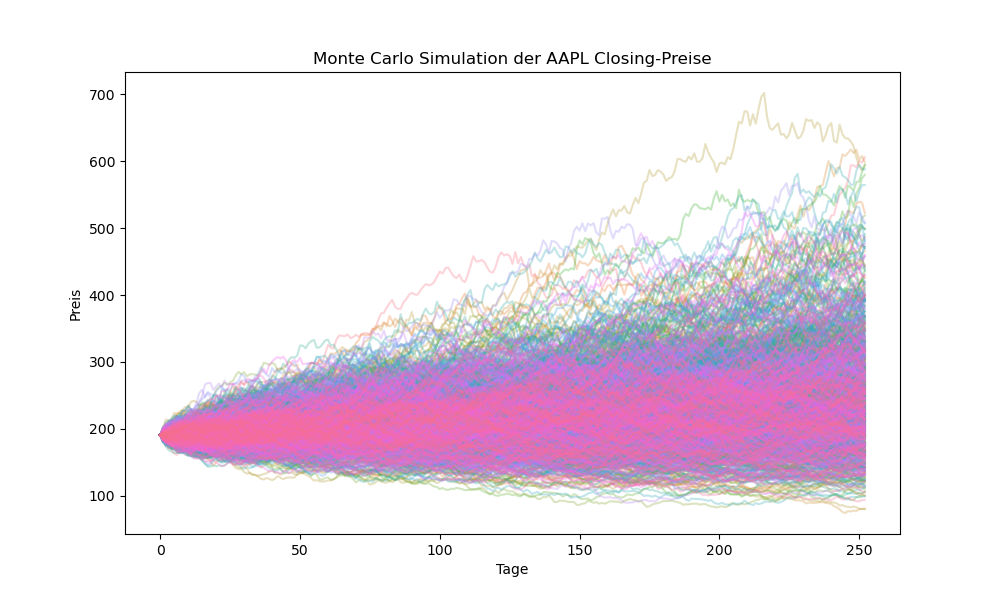
\includegraphics[width=\textwidth]{../Bilder/MonteCarloPlot.png}
    \end{minipage}
    \hfill
    \begin{minipage}{0.85\textwidth}
        \centering
        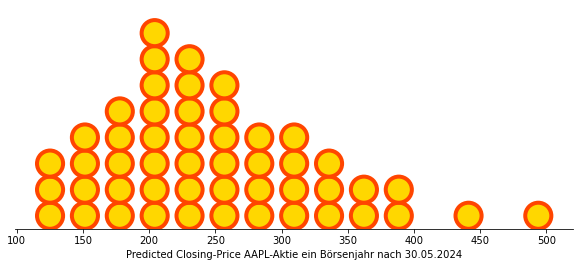
\includegraphics[width=\textwidth]{../Bilder/AAPL_QDP.png}
    \end{minipage}
    \caption{Gegenüberstellung herkömmliche Visualisierung vs. Quantile DotPlot}
    \label{fig:nebeneinander}
\end{figure}

\subsection{Diskussion}
Die Monte Carlo Simulation ermöglicht eine fundierte Analyse der zukünftigen Preisbewegungen der Aktie. Durch die Berechnung und Darstellung der Quantile können wir die Unsicherheiten und Risiken, die mit den zukünftigen Preisbewegungen verbunden sind, besser verstehen. Der Quantile Dotplot bietet eine visuelle Darstellung der Verteilung der Endpreise und hilft bei der Identifizierung der Wahrscheinlichkeiten verschiedener Szenarien. Dies unterstützt Investoren dabei, fundierte Entscheidungen zu treffen, indem sie ein besseres Verständnis für die Unsicherheiten und die potenziellen Risiken der zukünftigen Preisentwicklung der Aktie gewinnen.
Vergleicht man in Abbildung 1 die Verläufe der einzelnen Simualtionen augezeichent im Vergleich zu der Darstellung der Verteilung in einem Quantile Dotplot ist klar zu erkennen, aus welcher man eher die Tendenzen der zukünftigen Kursverläufe erkennen kann.

\section{Fazit und Ausblick}

\subsection{Zusammenfassung der wichtigsten Erkenntnisse}

In dieser Arbeit haben wir untersucht, wie sich die Visualisierung von Unsicherheiten und Risiken auf die Entscheidungsfindung auswirkt. Wir haben verschiedene Theorien zur Entscheidungsfindung unter Unsicherheit betrachtet, darunter die Erwartungsnutzentheorie und die Dual-Process-Theorie. Zudem haben wir die Bedeutung der Visualisierung von Unsicherheiten anhand einer Fallstudie im Bereich Fantasy Football untersucht. Es zeigte sich, dass Quantile Dotplots eine effektive Methode zur Darstellung von Unsicherheiten sind und die Entscheidungsfindung verbessern können.

Die Anwendung dieser Erkenntnisse auf die Finanzwelt wurde durch eine Monte Carlo Simulation für eine Aktienprognose demonstriert. Die Visualisierung der Ergebnisse mittels Quantile Dotplots zeigte die Verteilung der möglichen zukünftigen Preise und half, die Unsicherheiten zu quantifizieren.

\subsection{Proposal für künftige Forschung}

Für künftige Forschung schlagen wir vor, die Anwendung von Quantile Dotplots und anderen Visualisierungstechniken weiter zu untersuchen, um ihre Effektivität in verschiedenen Domänen zu bewerten. Insbesondere sollte erforscht werden, wie diese Techniken die Entscheidungsfindung in komplexeren finanziellen Szenarien unterstützen können. Darüber hinaus wäre es wertvoll, die Integration von maschinellen Lernmodellen und stochastischen Modellen zu untersuchen, um präzisere und robustere Prognosen zu ermöglichen. Ein weiterer Forschungsbereich könnte die Untersuchung der Benutzerfreundlichkeit und Verständlichkeit verschiedener Visualisierungstechniken für unterschiedliche Zielgruppen sein, um die Kommunikation zwischen Laien und Experten weiter zu verbessern.
